% !TEX root = sum1.tex
\section{Game Extension}
% 提到 pricing 会有固定的两/三个价格提供稳定
% 不存在 机器数量不变/scheduling的情况下, 可以稳定.
% 把证明没写的补充一下.

Then, we will try to extend the core concept to a more general case. So we need to define a new game as follow.

\subsection*{General model}

A cooperative TU game $(V,c)$ is a PIM(Price Integer Minimization) game if there exist:

\begin{itemize}
	\item positive integers e, v, t, P and m;
	\item integer vectors $ x \in \mathbb{Z}^{t \times 1} $and $ \tilde{\alpha} \in \mathbb{Z}^{1 \times t} $;
	\item left hand side matrix  $A \in \mathbb{R} ^{e \times t};$
	\item right hand side matrix $B \in \mathbb{R} ^ {e \times v};$
	\item a right hand side vector $D \in \mathbb{Z} ^ {e};$
	\item an objective function vector
	$c \in \mathbb{Z}^{1 \times t};$
	\item an incidence vector $y^s \in \{0,1\}^v$ with $y^s_k = 1$ if $k \in s$ and $y^s_k = 0 $ otherwise, $\forall k \in V$,

\end{itemize}

such that the characteristic function $c(s)$ equals the optimal objective value of the following integer linear program:

\[
c(s,P)= \mathop{\min}_{x} \{ cx+P\bar{m}(x): Ax \geq By^s+D, \tilde{\alpha}x \leq m, x \in \mathbb{Z}^{t \times 1} \}
\]

Note that the object function is not easy to analyze due to the joint effct of $cx$ and $P\bar{m}(x)$, we need to divide the function into two parts for a further discussion.

With the similar idea, we divide $c(s,P)$ as $c_0(s,m^*) + Pm^*$. Via the above analysis and study, we find some properties about $c_0(s,m^*)$ defined here.

If we want to get the non-overlapping price interval when the number of machines used changes, $c_0(s,m^*)$ must be supermodular, which corresponds to the following two lemmas.

\begin{lem}\label{price_positive}
% \\ \hspace*{\fill} \\ % 用于空行
% ~\\
\[c_0(V,m)- c_0(V,m-1) > 0 \Leftrightarrow P_m > 0, m=2,\ldots,n.\]
\end{lem}

\begin{lem}\label{non-overlapping}
\[
\begin{aligned}
&c_0 (V,m) - c_0 (V,m+1) < c_0 (V,m-1) - c_0 (V,m) \\
&\Leftrightarrow \quad P_m < P_{m+1} , m=2,3,\ldots,n.
\end{aligned}
\]
\end{lem}

Once the no-price characteristic function $c_0(s,i)$ be supermodular, we can specify this property in the following two aspects.
One is the concavity about the number of facilities,
the other is the nature about the number of players($s_1 \subset s_2$).
They correspond to the following two formulas:

\begin{equation}\label{concavity_f}
c_0(s_1,m-1)-c_0(s_1,m) \geq
  c_0(s_1,m)-c_0(s_1,m+1) \quad m=2,\ldots,n.
\end{equation}
% 只要这里是关于机器数量的变化即可
and

\begin{equation}\label{property_p}
	c_0(s_1,m-1)-c_0(s_1,m) \leq
	  c_0(s_2,m-1)-c_0(s_2,m) \quad m=2,\ldots,n.
\end{equation}
, respectively.

If the characteristic function satisfies the above property. Then $ P_1$ can be calculated by the following procedure:
When $\alpha(V) = c_0(V) + P_1$, which means the $\omega(P_1) = 0$. And the active inequalities must be the coalition contains $(n-1)$ players.
Then plus all the $(n+1)$ equality together, we can obtain $P_1 = (n-1)c(V)- \sum_{|s|=n-1,s\in S}c(s)$.
Because other inequalities will be satisfied according to the supermodular.

And shows that the number of using machines will not increase when the players increase.

Then we can develop the Theorem \ref{machine_num}.

\begin{thm}\label{machine_num}
When two coalitions $s_1,s_2$ satisfy $s_1 \subset s_2$, the corresponding number of using facilities $ m_{s_1}, m_{s_2}$ have $m_{s_1} \leq m_{s_2}$, if the primary function satisfies  (\ref{concavity_f}) and (\ref{property_p}).
\end{thm}

Although these conditions are rather harsh, IVPU and MSGW(which we are going to discuss in the following) game satisfies these properties clearly.

\subsection*{MSGW game}
Most analyses are applicable to the Machine Scheduling Game with Weighted jobs(MSGW).
In this game, each job $k \in V$ has a processing time, $t_k$, and a weight, $w_k$.
Note that the properties of this game is similar to the unweighted one, we will show main properties briefly in the following.

\begin{corollary} \label{cor-1}
$c(s,P)$ and $P_i(2 \leq i \leq v)$ can be obtained by analysing the order of $t_k/\omega_k$ instead of $t_k$.

\end{corollary}

\begin{corollary} \label{cor-2}
  $\omega(P)$ is piecewise linear, convex in price $P$ at each subinterval.
\end{corollary}

\begin{corollary} \label{cor-3}
  IPC, CP algorithms can be used to construct function $\omega(P)$ in polynomial time.
\end{corollary}

The notations, such as $c(s,P), \omega(P), P_i$ are the same as the above defined.

\begin{lem}\label{n-equality}
When $c_0(s,m^*), s \in S$ satisfy the supermodular and $P=P_1$, where we have $c_0(V,m^* = 1)$, $\alpha(s)=c(s, P_1), \left| s \right|= n-1$ and $\alpha(V)=c_0(V)+P_1$ the budget balance constraint holds. Meanwhile, the other coalitional stability constraints $\alpha(s) \leq c(s, P_1), \left| s \right| < n-1$ will hold.
\end{lem}

As we've already known that $P_i, i = 2,\ldots,n$ can be obtained by Lemma \ref{break_price}, then, $P_1$ can be calculated by solving the $n$ equalities by Lemma \ref{n-equality}.

Then we can follow the CP approach (Algorithm CP) to obtain all maximally unsatisfied coalitions the corresponding weak derivatives at each sub-interval $[P_{i+1},P_{i}]$ where the corresponding derivative is $m_V-\sum_{s\in S\setminus\{V\}} \rho_s$.

Then use IPC Algorithm which will return all the breakpoints during the $[0, P^*]$ to obtain the subsidy $\omega(P)$.

Remind that we want to realize a situation where the grand coalition doesn't need a subsidy from the externality.

Define the difference between the subsidy and the price increment on all machines used $D(P) = \omega(P) - \Delta P\cdot m^*(V)$. Initially, we have a initial price for every machine, then we set it as $P_0$.
According to \ref{dual}, the difference $D(P)$ can be expressed as $\omega^*(P) - (P-P_0)\cdot m^*(V)$. Meanwhile, together with Theorem \ref{w1P}, we know that all $m^*(s) =1$. Thus $D(P) = c_0(V, m^*(V)) + P_0 \cdot m^*(V) - \sum_{s\in S}\rho_s[c_0(s, 1) + P]$, which is still piecewise linear and convex at each sub-interval.

The figure is showed below.
\begin{figure}[h]%%图
	\centering  %插入的图片居中表示
	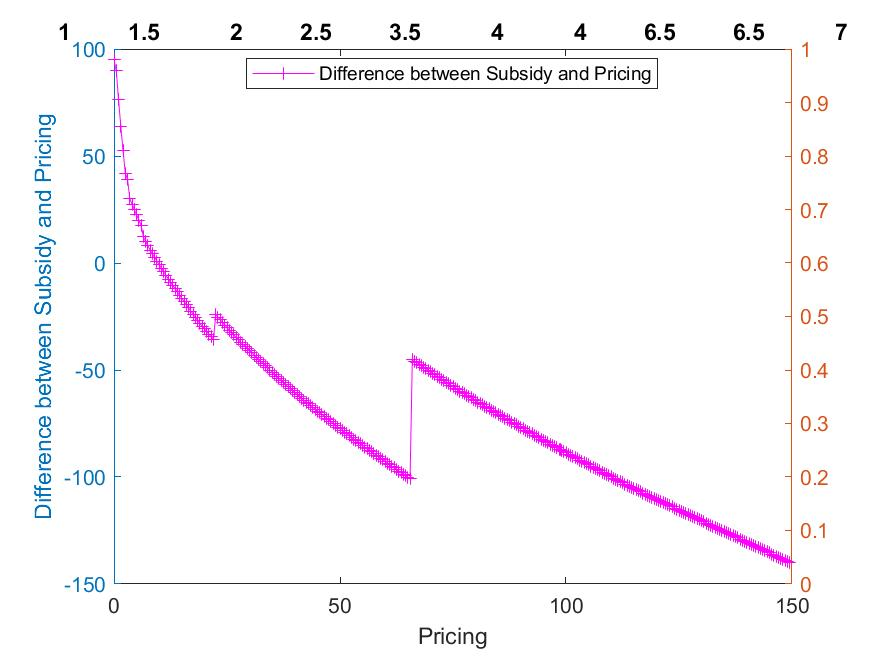
\includegraphics[width=0.8\linewidth]{Figures/Imagediff}  %插入的图,包括JPG,PNG,PDF,EPS等,放在源文件目录下
	\caption{The difference between subsidy and pricing increment}  %图片的名称
	\label{fig:Imagediff}   %标签,用作引用
\end{figure}

$D(P)$ is decreasing in every sub-interval, so it doesnot exist the situation where we do not need change the original schedule to stabilize the grand coalition.

Let $D(P) = 0$, then $c_0(V, m^*(V)) + P_0 \dots m^*(V) = \sum_{s \in S} \rho_s (P + c_0(s,1))$. However, $\{s\in S: \rho_s > 0\}$ which we need is very difficult to obtain.

If given an initial price $P_0$, we can use the dichotomy algorithm to calculate the solution of $D(P)$.

\begin{algorithm}[H]\label{algoDI}
\caption{The Dichotomy Algorithm to calculate the solution of $D(P)=0$.}
\begin{algorithmic}[1]
\begin{description}
  \item[Step 1.] Initially, given an initial price $P_0$, calculate the optimal scheduling and the number of machines used by the grand coalition $m^*$. \\
  \vspace{10pt}
  \item[Step 2.] Obtain the price interval $[P_{m^*+1},P_{m^*}]$ of the optimal scheduling. Calculate the corresponding subsidy $D(P_{m^*+1})$ and $D(P_{m^*})$, respectively. If $D(P_{m^*}) < 0$, continue Step 3. Otherwise, continue Step 4.
	\vspace{10pt}
  \item[Step 3.] Denote the price inverval $[a,b], a = P_{m^*+1}, b= P_{m^*}$ and the midpont $c =(a+b)/2$. Calculate $D(c)$, if the value is less than 0, let the interval be $[a, b=c]$, otherwise, the interval be $[a=c, b]$. Let $c =(a+b)/2$ again,
	continue this process until $D(c)$ is very close to 0, then we can get $P^{*} = c$.
  \item[Step 4.] Apply the similar method on the next interval $[P_{m^*},P_{m^*-1}]$
  \item[Step 5.] Return $P^{*}$.
\end{description}
\end{algorithmic}
\end{algorithm}

The algorithm gives the method to find the price to stabilize the grand coalition without externality.

There can exist one, two or three prices to achieve our goal, and commonly which depends on the value of processing time of all jobs.

Take this situation, optimal scheduling is using three machines, as an example, we need to consider the relationship of $P_1,P_2, P_3$.

Besides that, when the processing time is close to each other, we can conclude that the there exists two points to satisfy the requirement.
